\chapter{GPUHElib Design} \label{chap:GPUHElibDesign}
The first attempt at speeding up the run-time of HElib utilizes a GPU to parallelize operations. GPUs are often used to speed up computation where a single instruction or operation is performed on multiple pieces of data. GPUs are ideal for these types of designs because they allow for many compute cores to be run simultaneously, each performing the same operation. HElib utilizes a single instruction, multiple data (SIMD) design, however is single threaded. Meaning that, while being designed so that a single operation occurs over multiple data pieces, the library is not efficiently utilizing the design to best effect. The hope then of adding GPU functionality to the library is to thus take advantage of this design, by utilizing hardware that will best handle the SIMD nature of the scheme. 

There are three phases when executing operations on a GPU. First the memory is copied from the host(CPU) to the device(GPU). Then a kernel is created, which performs the operation on the data in the devices memory. Finally the data is copied back from the device to the host, upon which the host continues execution. The first and third phases are discussed further in Section \ref{sec:MemoryMapping}, and the kernel designs are addressed in Section \ref{sec:OverflowConsiderations}. Furthermore, these three phases can be parallelized to achieve the fastest speedup, discussed in Section \ref{sec:Pipelining}.

\section{Memory Mapping} \label{sec:MemoryMapping}
In order for the GPU to execute a kernel, it must have the data in a 1D vector. This requires that the data be mapped from its current storage model into a 1D vector.

\subsection{Mapping from CPU to GPU}

\begin{figure}[htp]
\centering
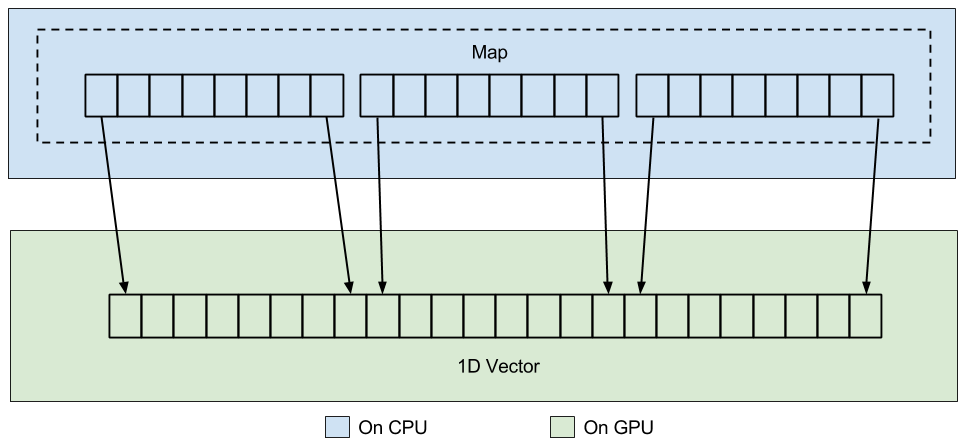
\includegraphics[width=0.65\textwidth]{MappingCPUtoGPUData.png}
\caption{Data Mapping from CPU to GPU}
\label{fig:MappingCPUtoGPUData}
\end{figure}

Currently the data is stored as shown in Figure \ref{fig:MappingCPUtoGPUData}. The \verb|map| contains vectors or rows, each of these rows are arrays of 64-bit integers. This structure is a non-contiguous 1D vector that needs to be mapped to a contiguous 1D vector. Thus the rows must be copied into a new vector, which the GPU will then operate on. Each successive row is concatenated to the preceding rows, thus creating a 1D vector.

\begin{figure}[htp]
\centering
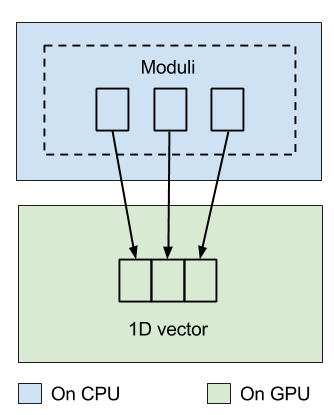
\includegraphics[width=0.3\textwidth]{MappingCPUtoGPUModuli.png}
\caption{Moduli Mapping from CPU to GPU}
\label{fig:MappingCPUtoGPUModuli}
\end{figure}

Similarly the moduli are being stored as individual elements. In order to be used during execution on the GPU, they must also be mapped to a 1D vector. Figure \ref{fig:MappingCPUtoGPUModuli} shows the current storage model for the moduli. Each successive modulus is concatenated to the preceding moduli, thus creating a 1D vector.

\subsection{GPU Vector Management}
Naively creating and freeing vectors on the GPU when the operation is run slows down run-times because allocating and freeing memory on the GPU takes time. Thus creating a few vectors at the beginning of execution, and maintaining them throughout the programs lifetime, allows for the most efficient memory usage, and greatest speedup.

Four vectors are created and maintained throughout the lifetime of the program. The first is a vector of size $num\_rows \times size\_of\_row$. This is the 1D vector that the data from the first \verb|DoubleCRT| object is being copied into. The second is another vector of size $num\_rows \times size\_of\_row$, which holds the data that is being copied from the other \verb|DoubleCRT| object. The third is a vector of size $num\_rows$. This vector holds the moduli. The last vector is also of size $num\_rows$, and is used when computing over a single \verb|DoubleCRT| object and a constant number. The constant number, modulus the moduli, are stored in this last vector. The sizes, $num\_rows$ and $size\_of\_row$, rarely change, thus there will be little memory reallocation occurring, and reallocation will only occur when the vector is too small, not when it is larger than needed. The function that handles initializing and reallocation of these vectors is found in Appendix \ref{sec:DeviceVectorManagement}.

\section{Overflow Considerations} \label{sec:OverflowConsiderations}
Arithmetic overflow occurs when the result of an arithmetic operation is greater than the magnitude of the storage location that is being used to store the value. For example, using 4-bit unsigned integers, the largest possible value that can be stored is $2^{4} - 1 = 15$. Thus when adding $12 + 14 = 26$, an overflow error will occur, because $26$ requires 5 bits to store. 

The type of the data being operated on in HElib is 64-bit signed integers. Meaning they can take values from $-(2^{63})$ to $2^{63} - 1$. However these values will never be negative, thus the actual range of these values is $0$ to $2^{63} - 1$. The largest modulus could be the largest possible value, $2^{63} - 1$ and the largest value being operated on could be $2^{63} - 2$. The reason that the largest value being operated on is one less than the largest value, $2^{63} - 1$, is because the value has to be smaller than the modulus, thus $(2^{63} - 1) - 1 = 2^{63} - 2$. In CUDA, the language used on NVIDIA GPUs, and the language this implementation is written in, the largest variable type has a length of 64 bits. The type that can contain the largest value is \verb|uint64_t|, unsigned 64-bit integers. This type can store values from 0 to $2^{64} - 1$.

Six operations were designed, as they are the most commonly used operations. Addition, subtraction, and multiplication of a \verb|DoubleCRT| with another \verb|DoubleCRT| and addition, subtraction, and multiplication of a \verb|DoubleCRT| with a constant number. Further considerations for overflow prevention for each operation is discussed in the following sections.

\subsection{Addition Overflow Considerations}
When considering the overflow prevention for addition, it is necessary to compute what the largest value could possibly be. As noted above, the largest a value could be is $2^{63} - 2$ and the largest modulus is $2^{63} - 1$. Performing the addition operation on the possible values, 
\begin{equation} \label{eq:add}
(2^{63} - 2) + (2^{63} - 2) = 2^{64} - 4
\end{equation}
shows that the number $2^{64} - 4$ needs to be computed, before the modulus operation takes place. This number is outside the range for signed 64-bit integers, but not for unsigned 64-bit integers. Thus the original numbers must be cast to unsigned 64-bit integers (which could cause problems if any of the numbers were negative, but since the values are always positive, there is no problem). After the addition operation takes place, the modulus operation brings the result back down the the range of signed integers, because the modulus is in the range of signed integers. The result is then finally cast back to a signed integer, and the operation is complete. The kernels for both addition operations, between two \verb|DoubleCRT| objects and between a \verb|DoubleCRT| object and a constant are in Appendix 
\ref{sec:KernelAddition}.

\subsection{Subtraction Overflow Considerations}
Similar to addition, it is necessary to compute the worst case scenario when considering overflow prevention for subtraction. Again the largest a value could be is $2^{63} - 2$ and the largest modulus is $2^{63} - 1$. There are two scenarios to consider for subtraction: the first number being $2^{63} - 2$ and the second number being 0 and the first number being 0 and the second number being $2^{63} - 2$. Performing the subtraction operation and modulus calculation for both scenarios,
\begin{equation} \label{eq:sub1}
(2^{63} - 2) - 0 = 2^{63} - 2
\end{equation}
\begin{equation} \label{eq:sub2}
0 - (2^{63} - 2) = -(2^{63} - 2)
\end{equation}
shows that all the computations can be completed using signed integers, because all numbers in the above equations are within the range of signed integers. Thus there does not need to be any steps taken to prevent overflow for this design. 

With this design, to ensure that the resultant value is greater than 0, a check is made after the subtraction operation takes place, to determine if the result is less than 0. If so, the modulus is then added to the value, which will result in the value being larger than 0. This check will cause a branch to occur in the GPU, which could slow down run-time. Alternatively, instead of performing a check to determine if the result is less than 0, the modulus can be added to the first value, then the second value is subtracted, shown in the below equation, which is a different approach to the subtraction operation. Equation \ref{eq:sub2} is redefined below, with this procedure applied. 
\begin{equation}
(0 + (2^{63} - 1)) - (2^{63} - 2) = (2^{63} - 1) - (2^{63} - 2) = 1
\end{equation}
Now when the modulus operation occurs, the correct result is found, however none of the values throughout the calculation were ever negative. Thus there is no need to perform a check, avoiding the branch, and possible slow down of the run-time. This method however does result in an overflow issue, because the modulus is being added to the first value. Below is this approach applied to Equation \ref{eq:sub1}.
\begin{equation}
((2^{63} - 2) + (2^{63} - 1)) - 0 = (2^{64} - 3) - 0 = (2^{64} - 3)
\end{equation}
This equation generates the value $2^{64} - 3$, which is too large for the signed integer range. Thus a similar procedure to that of addition is performed to ensure overflow prevention. The original numbers are cast to unsigned 64-bit integers. The operation detailed above takes place, before the modulus operation brings the result back down to the signed integer range. The result is then cast back to a signed integer, and completes the operation. The kernels for both subtraction operations, between two \verb|DoubleCRT| objects and between a \verb|DoubleCRT| object and a constant are in Appendix \ref{sec:KernelSubtraction}.

\subsection{Multiplication Overflow Considerations}
Multiplication presents much more problems compared to addition and subtraction. Again the largest value possible is $2^{63} - 2$, with the largest modulus being $2^{63} - 1$. Performing the multiplication operation on these values, 
\begin{equation} \label{eq:mul}
(2^{63} - 2) * (2^{63} - 2) = 2^{126} - 2^{65} + 4
\end{equation}
shows that very large numbers must be generated when performing the multiplication operation. Where for addition and subtraction the result could fit in a possible data type (unsigned 64-bit integer), these values will not fit in any data type available in CUDA. Therefore an algorithm must be used, which will break up the original numbers into smaller pieces. These pieces will then be used during intermediary steps to generate other values, that when combined back together will result in the correct answer, without ever generating a value that cannot fit in the GPU. The algorithm that is used is Karatsuba's algorithm. 

\subsubsection{Karatsuba's Algorithm}
\begin{equation} \label{eq:Karatsubas}
\begin{split}
x &= x_1 B^m + x_0\\
y &= y_1 B^m + y_0 \cr\\
z_2 &= x_1 y_1\\
z_1 &= x_1 y_0 + x_0 y_1\\
z_0 &= x_0 y_0 \cr\\
xy & = (x_1 B^m + x_0)(y_1 B^m + y_0)\\
 & = z_2 B^{2m} + z_1 B^{m} + z_0
\end{split}
\end{equation}

Equation \ref{eq:Karatsubas} shows Karatsuba's algorithm in general. The values being multiplied are $x$ and $y$. They are broken into pieces $x_1$, $x_0$ and $y_1$, $y_0$ respectively. These pieces are then used to create $z_2$, $z_1$, and $z_0$, which are finally combined with the base number, $B^m$, to generate the original result. For this case, $B=2$ and $m=32$. These values will ensure that operations performed throughout the execution of this algorithm never become greater than the maximum 64-bit unsigned integer value. Each of these will be examined more in-depth to see this.

When $x = 2^{63} - 2$, the variables $x_1$ and $x_0$ have values $x_1 = 2^{31} - 1$ and $x_0 = 2^{32} - 2$. The exact same values are assigned to $y_1$ and $y_0$ since $y = x = 2^{63} - 2$. 

Computing $z_2$,
\begin{equation}
\begin{split}
z_2 & = x_1 y_1\\
 & = (2^{31} - 1) (2^{31} - 1)\\
 & = 2^{62} - 2^{32} + 1
\end{split}
\end{equation}
shows that $z_2$ can fit inside a signed 64-bit integers, since the largest possible value is less than $2^{63} - 1$ (the largest value possible for signed 64-bit integers). 

Computing $z_1$,
\begin{equation}
\begin{split}
z_1 & = x_1 y_0 + x_0 y_1\\
 & = 2[(2^{31} - 1) (2^{32} - 2)]\\
 & = 2[2^{63} - 2^{33} + 2]\\
 & = 2^{64} - 2^{34} + 4
\end{split}
\end{equation}
shows that the intermediate pieces can be computed using signed 64-bit integers, however the addition operation causes the result to be in the range of unsigned 64-bit integers. Thus this calculation requires casting the pieces to unsigned 64-bit integers, carrying out the operation to calculate $z_1$, then performing the modulus operation to bring $z_1$ back down to the signed 64-bit integer space.

Computing $z_0$,
\begin{equation}
\begin{split}
z_0 & = x_0 y_0\\
 & = (2^{32} - 2) (2^{32} - 2)\\
 & = 2^{64} - 2^{34} - 4
\end{split}
\end{equation}
shows that $z_0$ must be calculated using unsigned 64-bit integers, since the result is too large for signed 64-bit integers. Thus this calculation also requires casting the pieces to unsigned 64-bit integers, performing the multiplication, before calculating the modulus to bring the result back into the signed 64-bit integer range.

Now that each of the intermediate pieces have been addressed, the final piece needs consideration. Computing $xy$,
\begin{equation}
\begin{split}
xy & = z_2 B^{2m} + z_1 B^{m} + z_0\\
 & = (2^{62} - 2^{32} + 1) (2^{64})\ +\ (2^{63} - 2^{34} + 5) (2^{32})\ +\ (2^{63} - 2^{34} - 3)
\end{split}
\end{equation}
shows that there will be problems computing $z_2 B^{2m}$ and $z_1 B^{m}$. However these can be dealt with deterministically. By performing a loop, multiplying $z_2$ and $z_1$ by 2, 64 and 32 times respectively, performing the modulus operation after every multiplication, one can obtain the correct value, without exceeding the unsigned 64-bit integer limit. Final modulus operations are applied to each addition, finally resulting in the correct value. This value is cast back to a signed 64-bit integer, and the operation is complete. The kernels for both multiplication operations, between two \verb|DoubleCRT| objects and between a \verb|DoubleCRT| object and a constant are in Appendix \ref{sec:KernelMultiplication}.

\section{Pipelining} \label{sec:Pipelining}
\begin{figure}[htp]
\centering
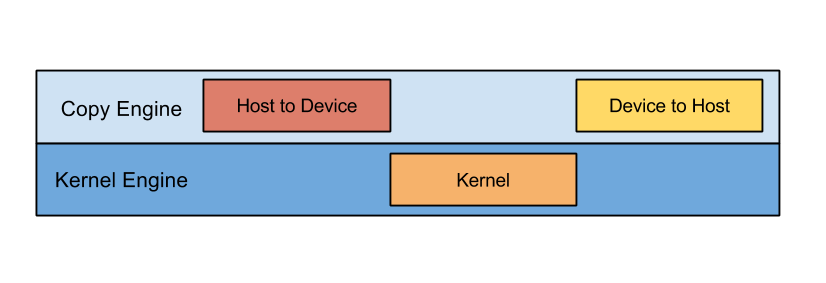
\includegraphics[width=0.65\textwidth]{GPUSerial.png}
\caption{Serial GPU Execution}
\label{fig:GPUSerial}
\end{figure}
As mentioned at the beginning of the chapter, there are three phases when performing operations on a GPU. First the data is copied from the host to the device, then the kernel is executed, and finally the data is copied back from the device to the host. The copy operations are handled by the copy engine, a processor that specifically deals with copying data back and forth from the host and device. Kernels are executed by the kernel engine. This operation is serial, meaning that all the data is copied from the host to device, before the kernel is executed. And the memory is not copied back, until all of the kernels have finished executing. This is illustrated in Figure \ref{fig:GPUSerial}. CUDA allows for these operations to be parallelized, using streams.

\subsection{CUDA Streams}
\begin{figure}[htp]
\centering
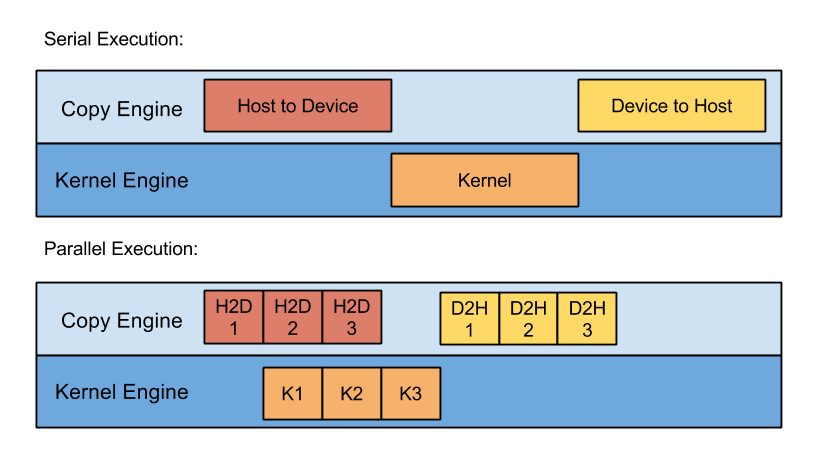
\includegraphics[width=0.65\textwidth]{GPUConcurrent.png}
\caption{Concurrent GPU Execution with 3 Streams}
\label{fig:GPUConcurrent}
\end{figure}
CUDA streams are a sequence of operations that execute in order on a GPU. Operations in different streams can execute concurrently, and be interleaved. Figure \ref{fig:GPUConcurrent}, shows this process applied to the same operations shown in Figure \ref{fig:GPUSerial}. One can see that this allows for speedup, because the copy to/from host to device can be executed, while the kernels are being executed. Streams are useful for parallelizing the computation, however the order in which the operations are dispatched also plays a role.

\subsection{Overlapping Kernel Execution}
There are two ways of dispatching GPU operations: all at once, or by batching similar operations together.

\subsubsection{All At Once Method}
The first approach launches all the operations at once, shown in Listing \ref{lst:AllAtOnce}.
\begin{lstlisting}[language=C++,caption={Operations launched all at once},label={lst:AllAtOnce}]
for (int i = 0; i < nStreams; i++) {
    int offset = i * streamSize;
    cudaMemcpyAsync(&d_a[offset], &a[offset], streamBytes, 
                    cudaMemcpyHostToDevice, stream[i]);
    kernel<<<streamSize/blockSize, blockSize, 
                0, stream[i]>>>(d_a, offset);
    cudaMemcpyAsync(&a[offset], &d_a[offset], streamBytes, 
                    cudaMemcpyDeviceToHost, stream[i]);
}
\end{lstlisting}
All three phases are launched successively on the same stream, before the next stream's operations are launched. 
\subsubsection{Batching Method}
The second approach is to launch similar operations together, instead of all at once. This is show in Listing \ref{lst:Batching}.
\begin{lstlisting}[language=C++,caption={Operations batched},label={lst:Batching}]
for (int i = 0; i < nStreams; ++i) {
  int offset = i * streamSize;
  cudaMemcpyAsync(&d_a[offset], &a[offset], streamBytes, 
                    cudaMemcpyHostToDevice, stream[i]);
}
for (int i = 0; i < nStreams; ++i) {
  int offset = i * streamSize;
  kernel<<<streamSize/blockSize, blockSize, 
            0, stream[i]>>>(d_a, offset);
}
for (int i = 0; i < nStreams; ++i) {
  int offset = i * streamSize;
  cudaMemcpyAsync(&a[offset], &d_a[offset], streamBytes, 
                    cudaMemcpyDeviceToHost, stream[i]);
}
\end{lstlisting}
In this second approach, all the copy from host to device operations are launched on their respective streams, then the kernels are executed, and finally the device to host copies are dispatched.

Both of these methods will produce the same result, as they are executing the same commands. However depending on the hardware being used, one method might achieve a better speedup over the other.

\subsection{2-Way Pipelining}
\begin{figure}[htp]
\centering
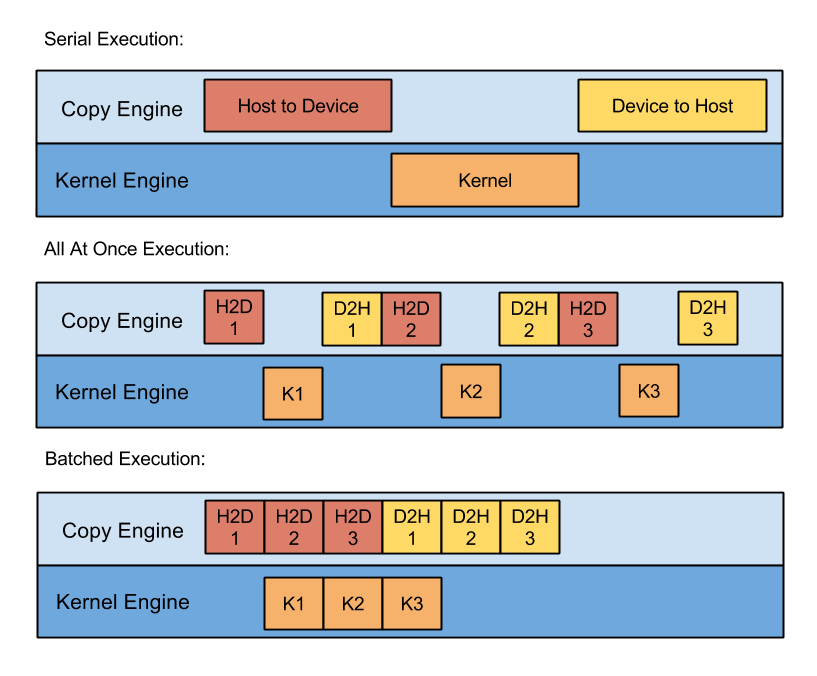
\includegraphics[width=0.65\textwidth]{GPU2Way.png}
\caption{GPU 2-Way Pipelining}
\label{fig:GPU2Way}
\end{figure}
Older GPU hardware only have a single copy engine and a single kernel execution engine. Figure \ref{fig:GPU2Way} shows both methods of kernel execution compared to serial execution. As one can see, both provide a speed up, however the batching method provides a greater speedup over the all at once method. This is because the all at once method launched the second copy from host to device after the first copy from device to host. Because there is only one copy engine, and the engine executes operations in the order they were launched, the copy engine must execute the copy from device to host, before the next host to device copy can occur. Using the second method though, the copies from host to device are all launched before the copies from device to host, so they call all execute one after the other. This allows for the most efficient pipelining, and the greatest speedup on hardware that only has one of each engine.
\subsection{3-Way Pipelining}
\begin{figure}[htp]
\centering
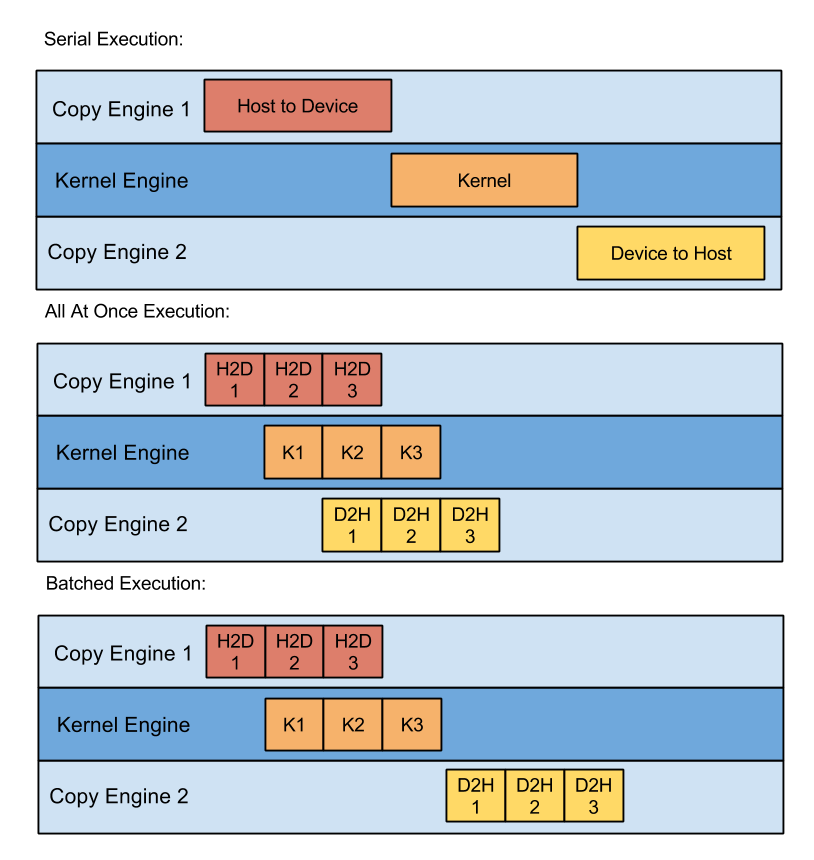
\includegraphics[width=0.65\textwidth]{GPU3Way.png}
\caption{GPU 3-Way Pipelining}
\label{fig:GPU3Way}
\end{figure}
Newer GPU hardware have both a copy from host to device engine and a copy from device to host engine, as well as the kernel engine. The two methods under this new hardware configuration are shown in Figure \ref{fig:GPU3Way}. Here one can see that again both methods provide an overall speedup, however for this case, the all at once method achieves the greatest speedup. Even though the first device to host copy was issued before the second host to device copy in the all at once method, the second host to device copy can be executed earlier than it because of the two copy engines. This is what is allowing the all at once execution method to be faster than the batching method. The batching method is suffering from a design choice in the scheduler of the GPU. The GPU tries to execute the kernels concurrently, and in doing so, delays a signal telling the device to host engine to starting copying until all the kernels have finished execution.

\subsection{Stream Management}
Naively creating and destroying streams as they are needed causes avoidable run-time slowdown. By managing the available active streams, one can achieve the most efficient design. For any instance of operation, the number of active streams is $num\_rows$ in the \verb|map|. This number will rarely change, thus initially creating $num\_rows$ amount of streams, and only creating more streams when there are not enough, efficiently maintains the fewest amount of needed streams at all times. Appendix \ref{sec:DeviceStreamManagement} contains the functions used to manage the streams.